\chapter{INTRODUÇÃO}
A manufatura aditiva emerge como uma tecnologia altamente promissora para a produção de peças e componentes em diversas áreas, incluindo engenharia, medicina e a indústria aeroespacial. Suas características distintivas viabilizam a fabricação de peças complexas em pequenas quantidades, promovendo uma notável iterabilidade, bem como suportando a produção descentralizada sob demanda. Nesse contexto, a impressão 3D, em particular o método de "Fused Deposition Modeling" (FDM), ganha destaque crescente, encontrando aplicações variadas nos setores aeroespacial, automobilístico e prototipagem rápida, ao mesmo tempo que se torna mais acessível e disseminada.

A modelagem digital desempenha um papel essencial no processo de impressão 3D, trabalhando em conjunto com ferramentas como o "Computer Aided Design" (CAD). Essa parceria possibilita a criação de modelos tridimensionais altamente precisos, que podem ser compartilhados e reproduzidos de forma descentralizada. Quando se trata de imprimir um desses modelos, a preparação é realizada através de um software de fatiamento, conhecido como "slicer". O slicer divide o modelo em camadas e gera os comandos necessários para a impressora 3D. A impressora, por sua vez, interpreta esses comandos para determinar como proceder e quando executar cada ação. É importante notar que entre a interpretação e a execução desses comandos existem diversos processos intermediários que exercem influência direta sobre a qualidade e a velocidade da impressão.

\begin{figure}[H]
    \begin{center}
    \caption{Fluxograma etapas Impressora 3D FDM}
    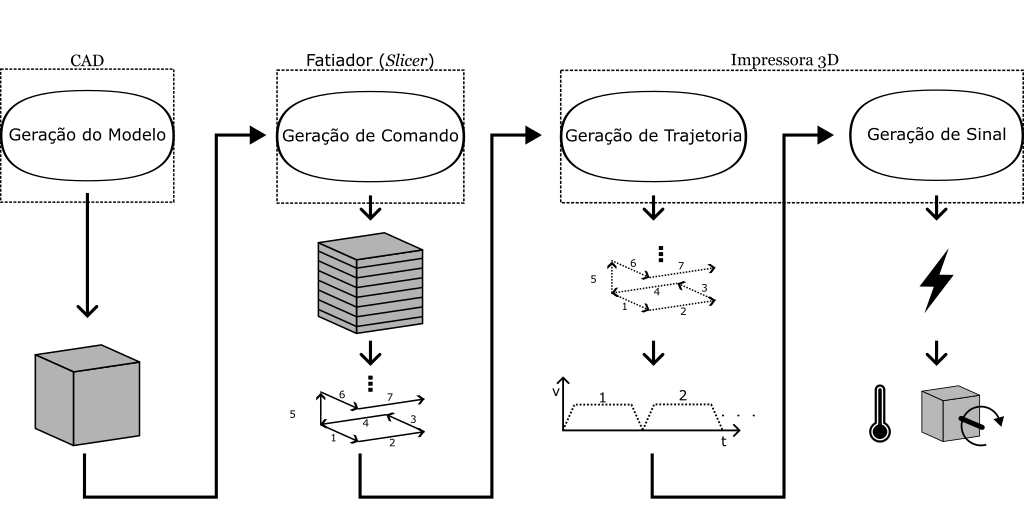
\includegraphics[scale=0.55]{flowchart_intr}

    \label{fig:flowchart_intr}
    \end{center}
\end{figure}

No entanto, uma das limitações significativas da impressão 3D, especialmente do tipo FDM, é o tempo de 
impressão, que ainda restringe o tamanho das peças produzidas em um período razoável. Frequentemente, é 
necessário utilizar camadas e linhas mais grossas para compensar esse aspecto, diminuindo a habilidade de
se reproduzir detalhes menores. Diante disso, existe uma procura por maneiras de se imprimir mais rapidamente, 
sem comprometer a qualidade.

Assim, é relevante explorar técnicas que permitam alcançar capacidades superiores de qualidade e 
velocidade de impressão, flexibilizando a tecnologia e ampliando sua aplicação comercial viável. 

Este trabalho tem como objetivo investigar e desenvolver uma metodologia para atuação de controle na geração de
comandos em impressoras 3D utilizando o método FDM de forma a possibilitar maiores velocidades e garantindo a precisão dimensional das peças produzidas.